\documentclass[msthesis.tex]{subfiles}

\begin{document}
\chapter{Results}
In this section, the quantitative and visualization results from the methods presented in the chapter \ref{chap:methods} will be presented. The first two sections will present results from preprocessing of the DWI images mentioned in \autoref{sec:Diffusionimgprepro} and extraction of connectivity matrices. The next sections will statistically describe the nature of the data as well as classification results based on the comprehensive classification parameters explained in \autoref{tab:classify_combo}.

\section{Preprocessing Visualization}
\begin{figure}
    \centering
    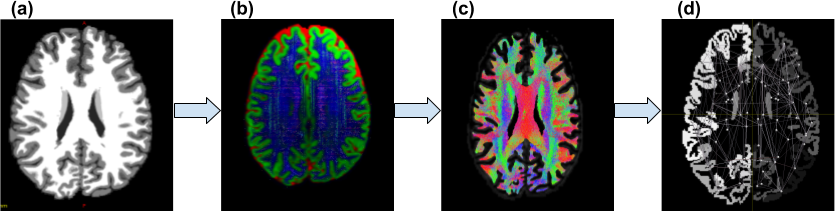
\includegraphics[width=\textwidth]{images/Preprocessing_pipeline.png}
    %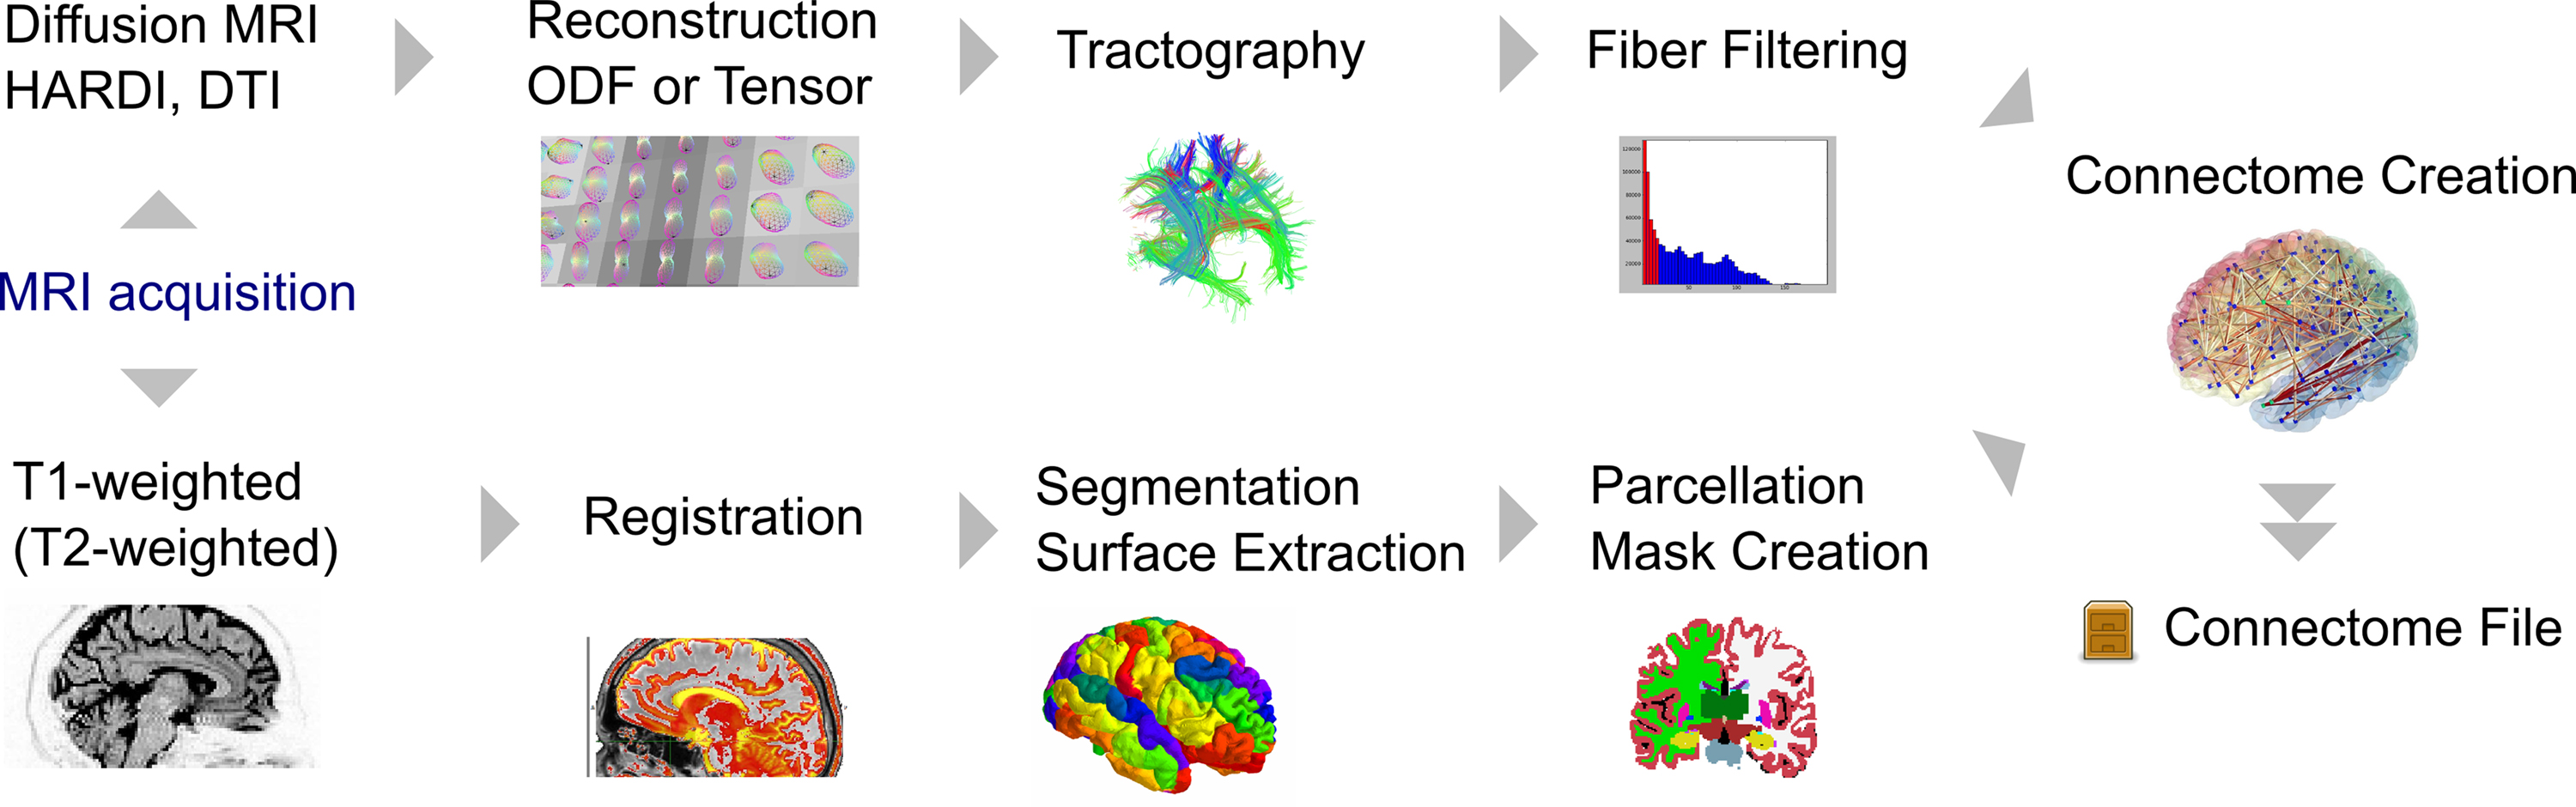
\includegraphics[width=\textwidth]{images/connectome_creation_workflow.png}
    %\cite{gerhard2011connectome}
    \caption{Visualization of pipeline used to create a connectome for each subject (a) Five tissue segmented image visualized in grayscale. (b) A slice of a 4D image mapped in 3D using RGB encoding tissue densities, CSF as red, GM as green and WM as blue. (c) Anatomically constrained tractography (ACT) of one million fibers overlaid on an axial slice of the brain. (d) The nodes of the connectome representing ROIs overlaid on an axial slice}
    \label{fig:preproc}
\end{figure}

During the process of generating the connectome (\autoref{subsec:connectomegeneration}) visual inspection was required to investigate the properties of different types of images produced. The results illustrated in \autoref{fig:preproc} used to evaluate the adherence of the implementation to the conceptual framework mentioned \autoref{sec:creating_connectome}. 

The 5TT image obtained after tissue segmentation (\autoref{subsec:struct_diff}) was 4D and could not be easily displayed in 3D. In \autoref{fig:preproc}.a, this 4D image is displayed according to gray-scale mapping in 3D. With the grayscale mapping it was viusally observed that the 5TT images did not contain any erroneous labels. The original 4D image contained three volumes with each one representing the corresponding tissue densities of WM, GM and CSF. In \autoref{fig:preproc}.b. the 5TT 4D image is visualized as an RGB image with each volume getting its specific color, i.e. WM as blue, GM as green and CSF as red. In interactive window from \textbf{\textit{mrview}} (\cite{tournier2019mrtrix3}) the RGB image can be zoomed in an checked for compliance of the response functions with the fODFs and tissue segmentations. 

After obtaining information about the tissue segmentations and fODFs, one million fibers whole brain tractography was generated (\autoref{fig:preproc}.c). In this tractogram, the red fibers run in right to left direction, green between anterior-posterior and blue in head-to-foot direction (\cite{obert2013evaluation}). Finally, the connectome could be visualized (\autoref{fig:preproc}.d) with the nodes representing the center of mass of grey matter regions and edges as the connections between them. The intensity of this image is not equal to the signal intensity but the number assigned to the ROI, so any parcellated region that has a higher numbering in the lookup table is shown brighter. However, the diagram still remains informative. 

Overall, visualizing the preprocessing pipeline helped to evaluate the anatomical correspondence of the tractography. It also helps understand the relationship between the generated connectome and white matter connectivity.

\section{Connectome Visualization}

\begin{figure}
    \centering
    %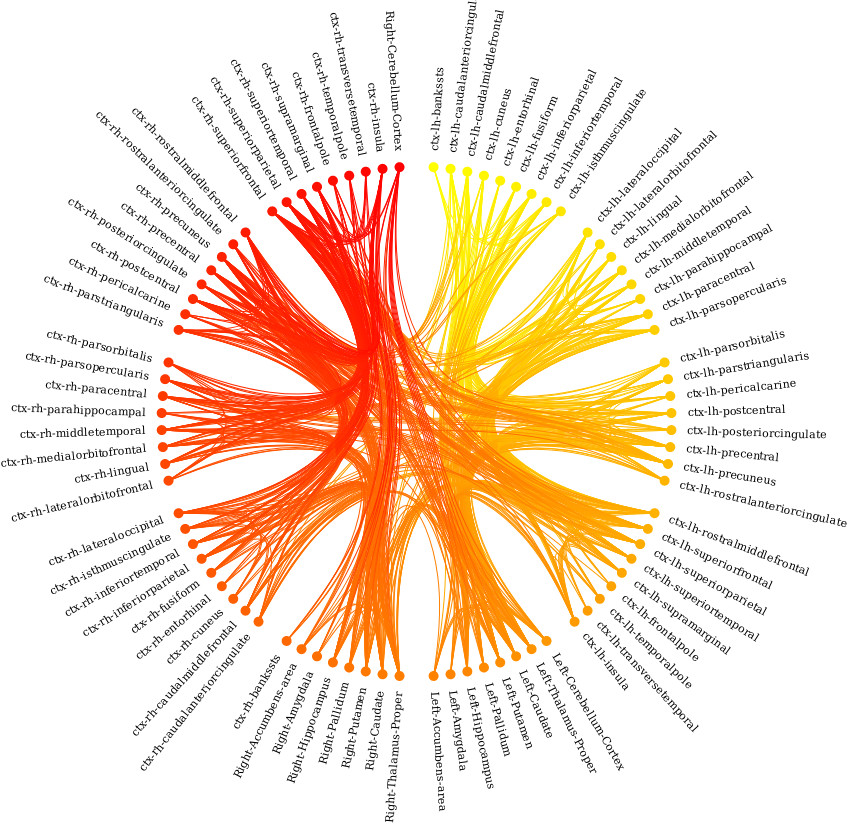
\includegraphics[width=\textwidth]{images/brain-data-viewer_2.png}
    %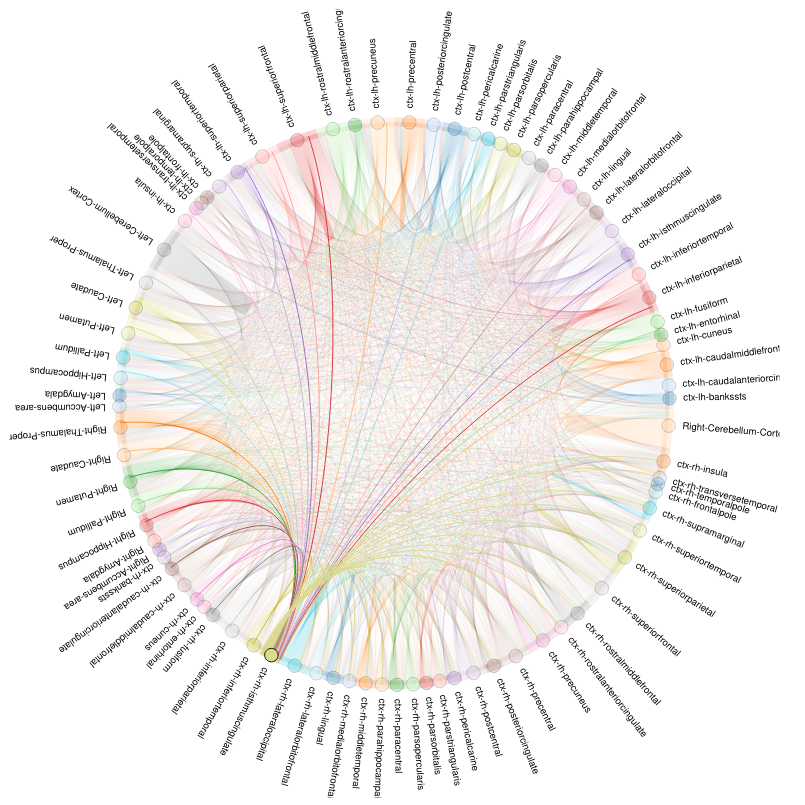
\includegraphics[width=\textwidth]{images/bokeh_plot_allsubjects.png}
    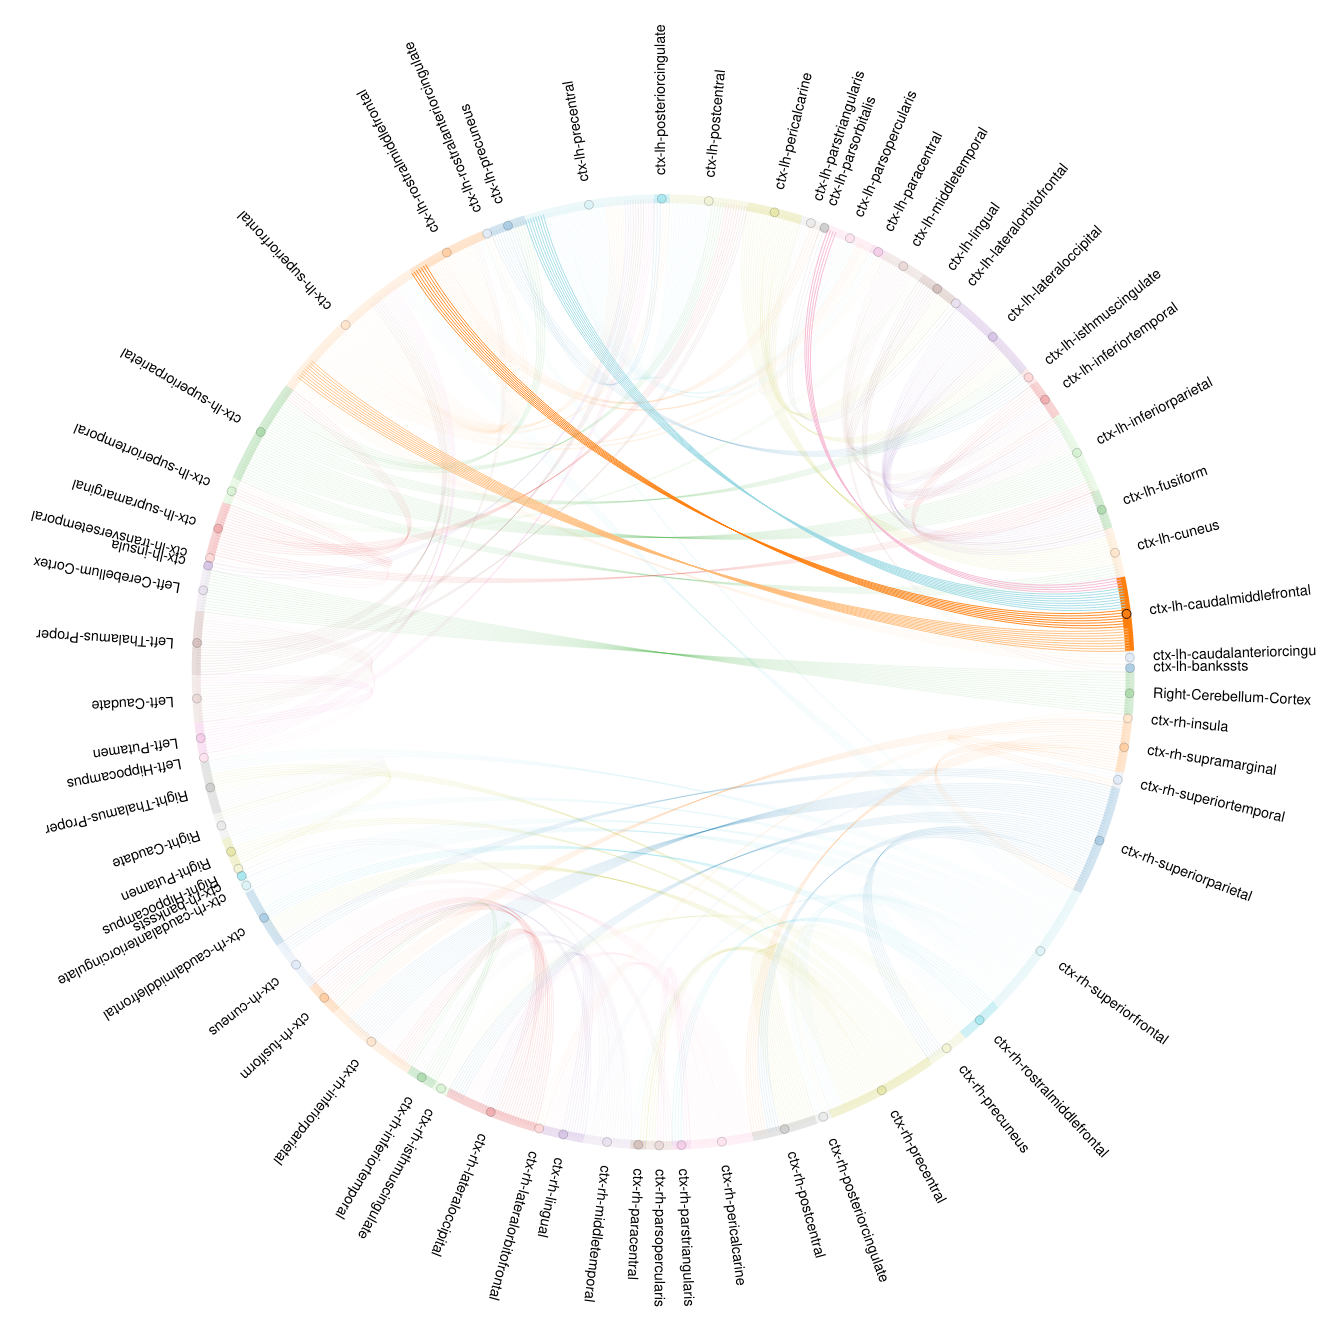
\includegraphics[width=\textwidth]{images/selected_view_all.png}
    \caption{A chord plot representing the group averaged connectome for all subjects. The number of arcs (edges) represent the number of streamlines between any two ROIS. The ROIs are represented as the nodes in the diagram at the end of the circle. The presence of multiple arcs get bundled together and increased multiple arcs are represented by one arc with higher thickness. The middle frontal gyrus in the left hemisphere is selected as the source node and the all the edges convergent on this node are colored according to the terminal node.}
    \label{fig:connectome_num_streamlines}
\end{figure}

After the connectivity matrices for all subjects were generated using methods in \autoref{sec:creating_connectome}, the group averaged connectome was created. The raw connectivity matrix was dense, containing $n = 84$ nodes and $n_e = 3486$ edges. The edge weights were widely distributed for the different types of features. Visualizing the connectome as a simple connectivity matrix or a heatmap was hence not an effective strategy.

A chord plot was chosen because of the organization and structure, ease of representing grey matter nodes. The number of streamlines served as a suitable connectivity metric to be encoded into a chord plot, the reason for the selection of the number of streamlines will be presented in \autoref{subsec:connmetric}. The detailed coloring scheme used for creating the chord plot gives added visual cues about the source and the target nodes.

In the chord plot represented in \autoref{fig:connectome_num_streamlines} $n=65$ nodes are shown. The graph is obtained by thresholding the group averaged number of streamlines between any two ROIs. The threshold was selected to be $N=900$ and the value for thickness of the arc was deciding by dividing the preserved number of streamlines by a factor of 10. For interactive visualization, the cortical region caudal middle frontal in the left hemisphere is selected. Its has prominent connections to the cortical regions superior frontal, rostra middle frontal and precuneus in the left hemisphere. Weak connection to the cortical region parsopercularis is also well represented by this diagram. 

Overall, this comprehensive diagram is a systematic representation of whole brain connectivity. It can be used to analyze brain connections at the subject level or the group level.

\section{Feature Analysis}

Once the connectivity matrices were ready, it was important to investigate an effective connectivity metric and determine importance of within ROI connections. From the preprocessing pipeline presented in \autoref{sec:connectome_generation} there were three types of connectivity metrics obtained for each subject. These were number of streamlines, the mean streamline length and the mean FA. Each of these features encodes a different biological property of between ROI connections and gave different classification results. There is no current consensus on which feature qualifies as an effective measure of connectivity between any two nodes (\cite{yeh2020mapping}). The number of streamlines was selected to be the major focus of the classification tasks due its superiority in classification performance, which will be illustrated subsequently. Further, exclusion of self loops from the connectivity matrices will be experimentally justified. 

\subsection{Differences in connectivity metric}
\label{subsec:connmetric}
\begin{figure}
    \centering
    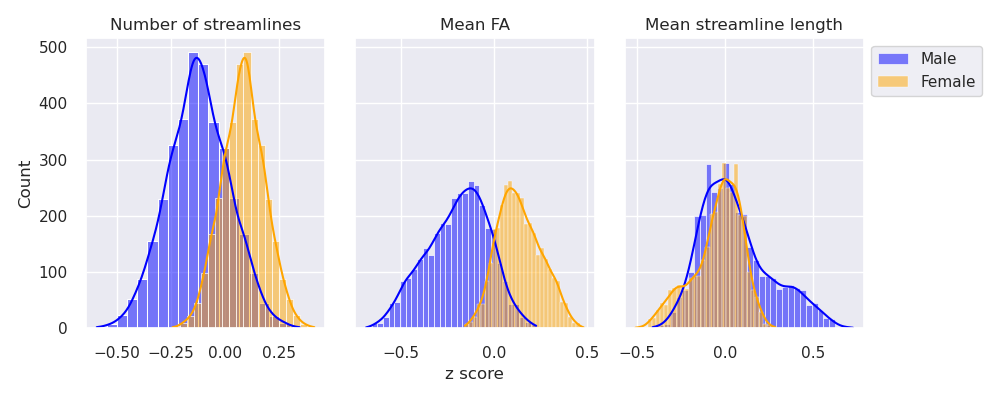
\includegraphics[width=\textwidth]{images/zscoredist.png}
    \caption{Three overlaid histograms representing the frequency of mean z scores for different types of features. The orange histograms are for females and blue ones are for males.the y axis represents the number of between ROI connections.}
    \label{fig:hist_zscores}
\end{figure} 
As mentioned above, it was important to explore different types of connectivity metrics obtained from the connectivity matrices constructed using methodology \autoref{fig:hist_zscores}. Considering the z score distributions of ROI connections separately for males and females was taken as a method for data evaluation. A histogram for the three different feature or connectivity types could help speculate which one performs better while classifying target variables/ or how well they could separate between the two classes.

The histograms were formed using data (containing both males and females) from the training set. Each feature was then standardized by removing the mean and scaling it to unit variance. After scaling the feature value for each subject is represented by a z statistic. The mean of the z statistic (of one feature) is zero for all training subjects. However, the differences are prevalent when separate means are taken for the two genders. For each connection, there was one z score for males and another for females depending on the connectivity metric. For each connectivity metric there are 3486 features which help form the distribution represented in \autoref{fig:hist_zscores}.

From the distributions, it is evident that the number of streamlines is a superior connectivity metric for gender classification. It's histogram is non-overlapping, shows a smooth Gaussian distribution for males and females, and has significantly higher peaks than those for the other two features. From the differences in z-score distribution, it can be inferred that women on an average have more number of streamlines as compared men, for the same connections. This observation is coherent with evidence in  \cite{szalkai2015graph} showing that women have more densely connected brains than men. Further, women have higher white matter to grey matter ratio and hence the number of streamlines detected for women is higher \cite{taki2011correlations}.

Using the mean FA plots illustrate that women have higher mean FA values than men. Conversely, an opposite trend is seen in the case of mean streamline length. Women have lower z scores, which points that shorter streamline lengths. There are yet no conclusive results for benchmarking such a distribution as gender differences prevail depending on ROIs being considered (\cite{kanaan2012gender}).For the mean FA, it is difficult to conclude that female brains have higher FA values when considering whole brain connectivity existing studies do not provide conclusive results (\cite{ingalhalikar2014sex}). The shorter streamline lengths in women seem plausible since, on an average women's brains are smaller than that of men (\cite{ankney1992sex}).

The results for the number of streamlines and the mean streamline length are coherent with \textit{a priori} knowledge and evidence in literature. These features could have contained biases as the tractography was carried out in individual subject's space. Comparing the streamline count or length for different subjects was possible due to the informed filtering using the SIFT algorithm (\cite{yeh2020mapping}).

The experiments stated above help establish the effectiveness of streamline count as a connectivity metric. It can well discriminate between gender and gives a biologically coherent
measure of brain connectivity.

\subsection{Self loops}
\label{res:selfloops}

The results for the experiment mentioned in section \ref{sec:exclusion} are presented in table \ref{table:selfloops}. For the independent test data all p-values are $p>0.05$ and the t statistic values represent the differences in the classification metrics with and without the inclusion of self loops. The low absolute values of the t-statistic further increased the evidence for insignificance of inclusion of self loops for classification accuracy.

\begin{table}
\label{table:selfloops_combined}
\csvreader[
  tabular=|p{0.13\textwidth}|p{0.15\textwidth}|p{0.29\textwidth}|p{0.08\textwidth}|p{0.09\textwidth}|,
  table head= \specialrule{0.2em}{0.05em}{0.05em} Target Label & Metric & Feature & T test & P value\\ \hline,
  late after last line=\\\hline,
]{tables/Combined_self_loops.csv}{}%
{\csvcoli  & \csvcoliii & \csvcoliv & \csvcolv & \csvcolvi}
\caption{Results for a paired samples t-test carried where paired samples are the classification metrics of the data with and without the inclusion of self loops. The corresponding p values are for two arrays for the same classification metric with each array representing classification metric for the five different personality traits. Based on test data only.}
\end{table}

\section{Baseline analysis}
\begin{figure}
    \centering
    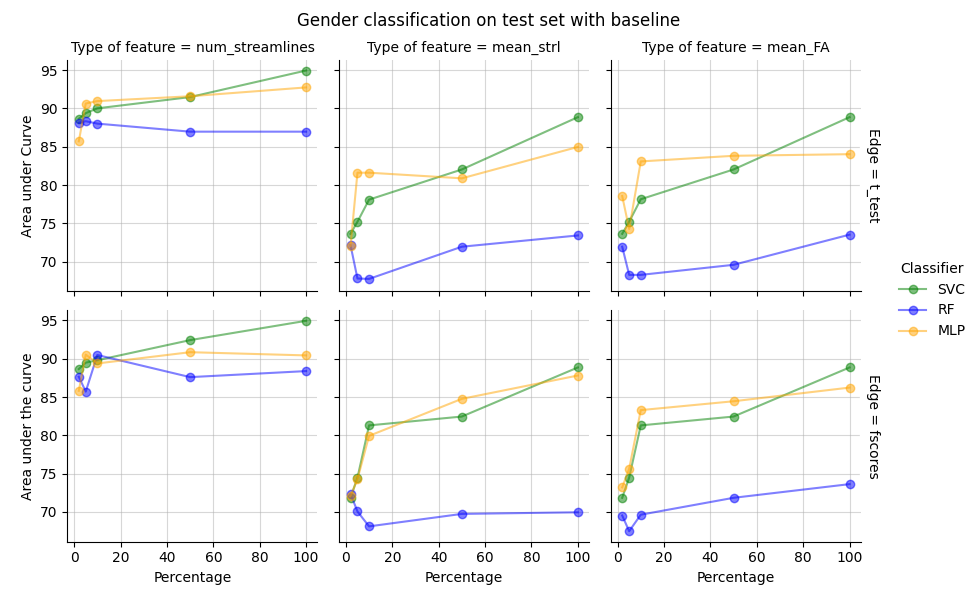
\includegraphics[width=\textwidth]{images/baseline_results_gender.png}
    \caption{Baseline analysis for gender classification. The area under the curve represented as a function of percentage of features. }
    \label{fig:my_label}
\end{figure}
\begin{figure}
    \centering
    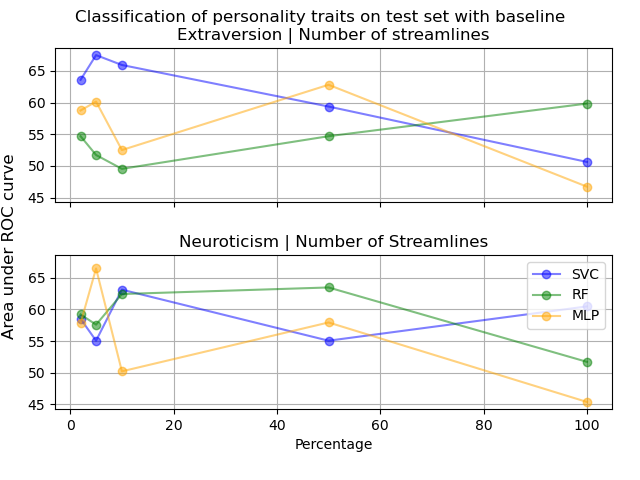
\includegraphics[width=0.8\textwidth]{images/persona_2.png}
    \caption{Baseline analysis on the basis of personality traits using pearson correlation coefficient. In a general trend it can be seen that doing some feature selection is beneficial for the classification.}
    \label{fig:persona base}
\end{figure}
In the baseline analysis choosing the number of streamlines with any type filter methods still retains most of the classification information. There is not much reduction in the AUC from using all the features until retaining only a small subset of features.

For both the personality traits and the gender based classification, feature selection seems profitable in terms of going towards interpretability. For the personality based classification which is a tough task doing this was difficult and hence....

\subsection{Solver}
After filtering according to the edges being selected only when there is at least one streamline per subject. On the basis of the training subjects, the number of features for which all the subjects have a at least one streamline with them is 1150. The input graph is hence formed on the basis of this with this number determining the upper bound of the number of edges in our input graph. 

In Fig. \ref{fig:gender_num_strls_10} the MEWS solver based implementation reduces the input graph based on the fscores to infer the most important set of connections. In this graph the edges obtained from Fig. \ref{fig:solver_based_gender_10} were traced back to the original \textit{dataframe} containing the data about number of streamlines for all subjects. The number of streamlines between the regions delineated were determined to put together in the chord graph. From the thickness of the arcs in the chord graph the Left-Palladium and right thalamus proper seem to have the maximum number of connections between them. Further, the subcortical regions seem to have more number of streamlines between them than the cortical regions. 


\begin{figure}
    \centering
    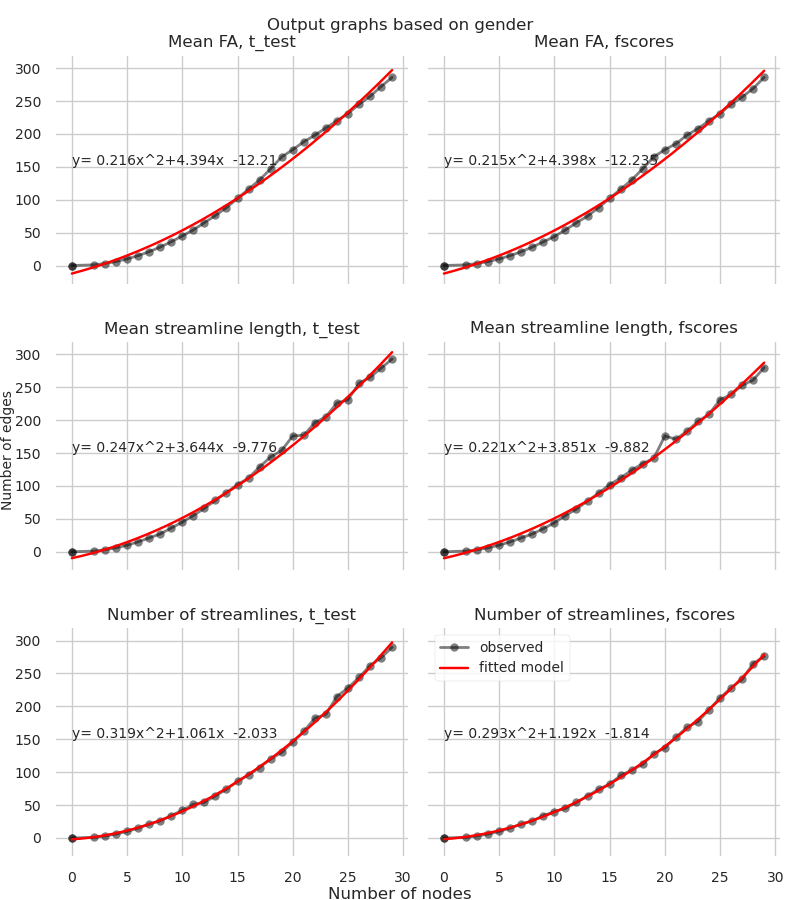
\includegraphics[width=0.8\textwidth]{images/Gender_nodes_preserved.png}
    \caption{Edges preserved as a function of nodes in the case of gender subgraph reduction}
    \label{fig:fun_num_edges}
\end{figure}

\iffalse
\begin{figure}
    \centering
    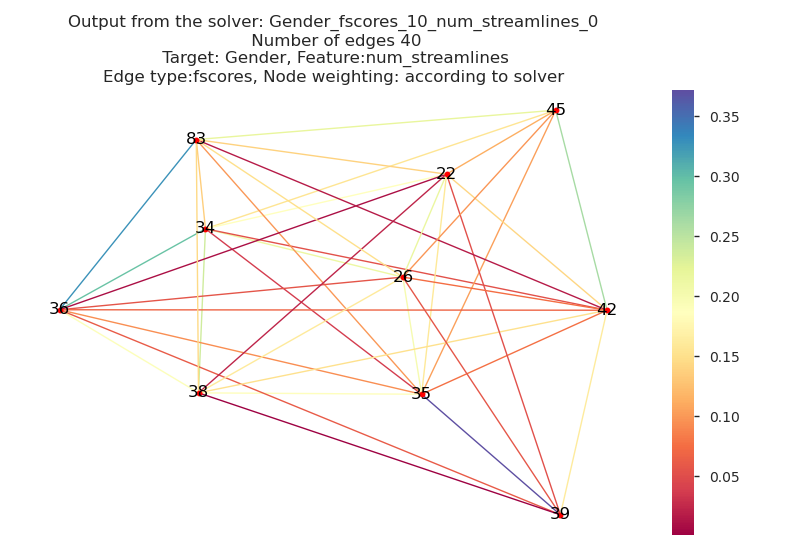
\includegraphics[width=0.5\textwidth]{images/gender10nodes.png}
    \caption{Caption}
    \label{fig:solver_based_gender_10}
\end{figure}

\fi

\begin{figure}
    \centering
    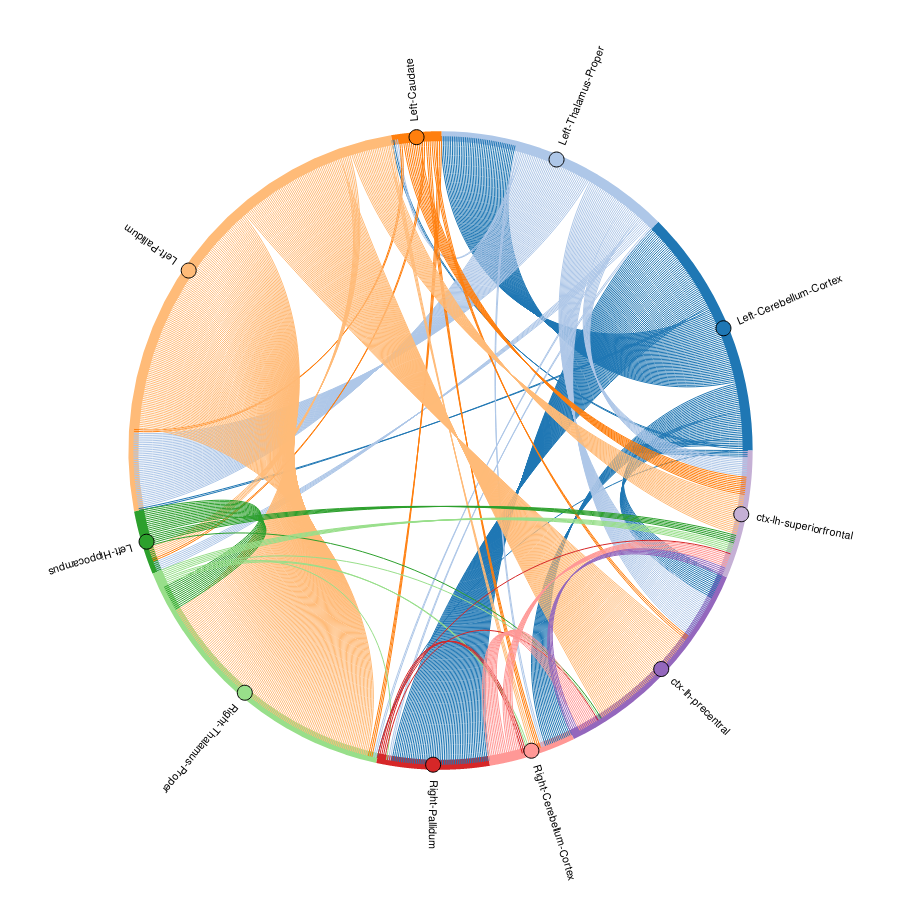
\includegraphics[width=0.9\textwidth]{images/gender10nodes_numstrls.png}
    \caption{10 most important nodes determined using the solver based analysis using the fscores for the Gender based classification. This graph is a Chord graph implemented using Holoviews (\cite{stevens2015holoviews}). The number of edges between any two nodes represent the number of streamlines between them. The fscores were used in order to determine the importance of the connections, the filtered edges retraced back to the original matrix yielded this result. The number of streamlines was averaged for all subjects and then the filtered edges based on the solver were produced. Multiple edges are drawn in the chord type graph where the number of edges represents the number of streamlines.}
    \label{fig:gender_num_strls_10}
\end{figure}


For the features determined by the subgraph. The reduced features were put through an independent samples t-test for gender differences. 


\begin{table}
\label{table:10strls_gender}
\csvreader[
  tabular=|c*{4}{|c}|,
  table head= \hline feature & ROI & ROI & P value\\ \hline,
  late after last line=\\\hline,
]{tables/gender10_numstrls.csv}{}%
{\csvcoli & \csvcolii & \csvcoliii & \csvcoliv }
\caption{Results for an independent samples t-test carried, The corresponding p values are for the different number of streamlines for males and femalestvod .}
\end{table}



\iffalse
\begin{figure}
    \centering
    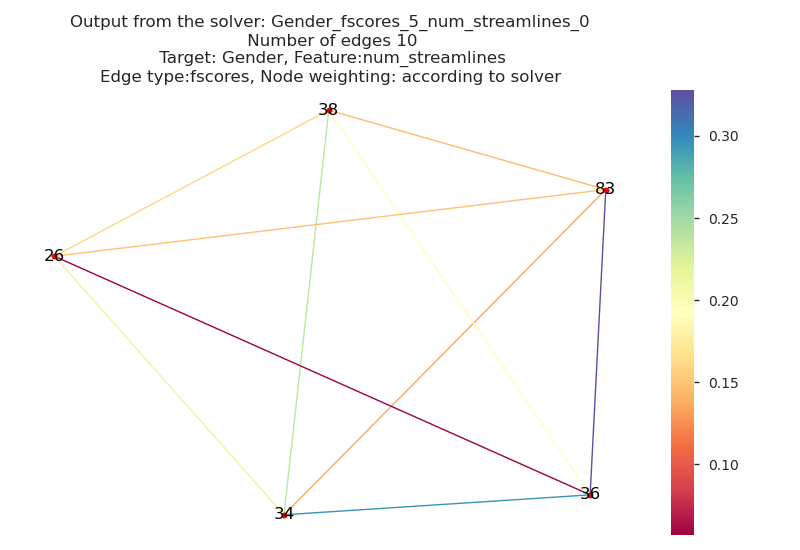
\includegraphics[width=0.8\textwidth]{images/Gender5nodes.png}
    \caption{Caption}
    \label{fig:}
\end{figure}

\begin{figure}
    \centering
    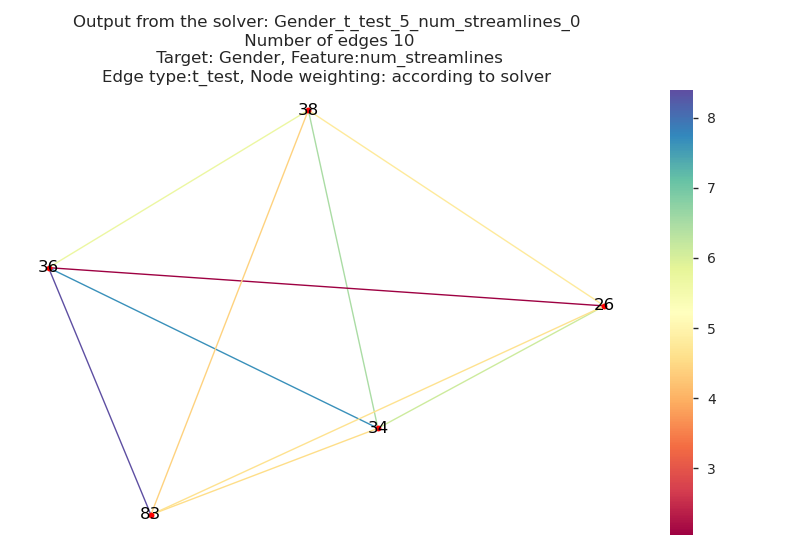
\includegraphics{images/Gender5nodes_test.png}
    \caption{Caption}
    \label{fig:my_label}
\end{figure}
\fi
\iffalse
\section{Solver and baseline comparison}
\begin{figure}
    \centering
    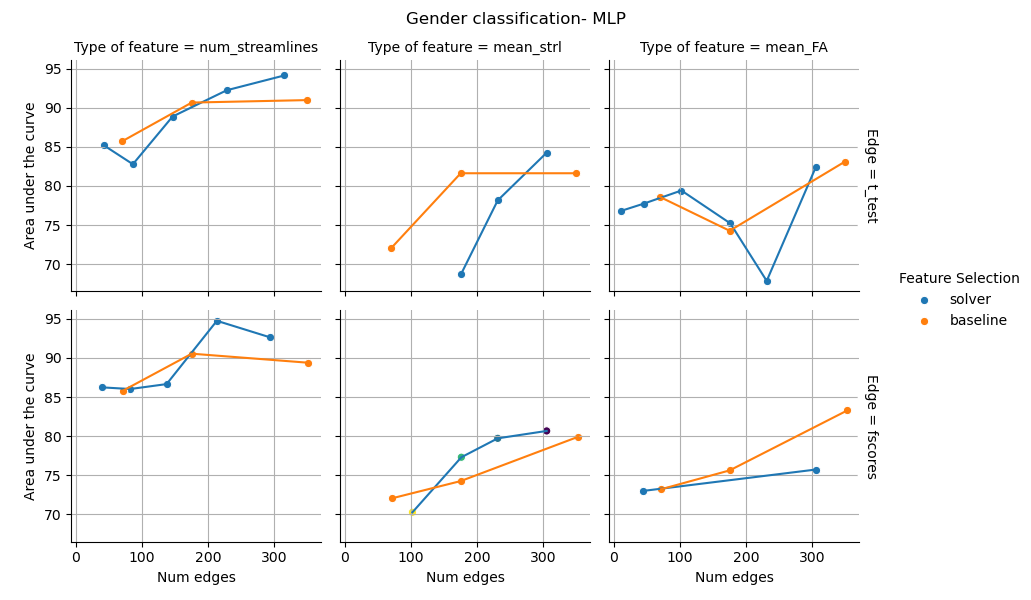
\includegraphics[width = \textwidth]{images/comparison_roc_auc_MLP.png}
    \caption{Caption}
    \label{fig:mlpgender}
\end{figure}
\begin{figure}
    \centering
    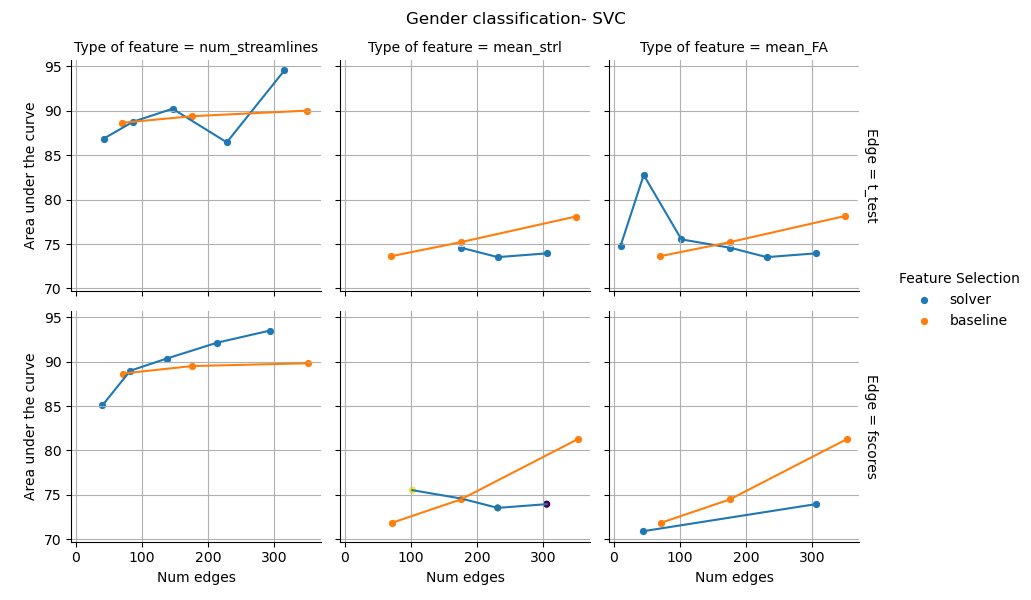
\includegraphics[width = \textwidth]{images/comparison_roc_auc_SVC.png}
    \caption{Caption}
    \label{fig:svcgender}
\end{figure}

\begin{figure}
    \centering
    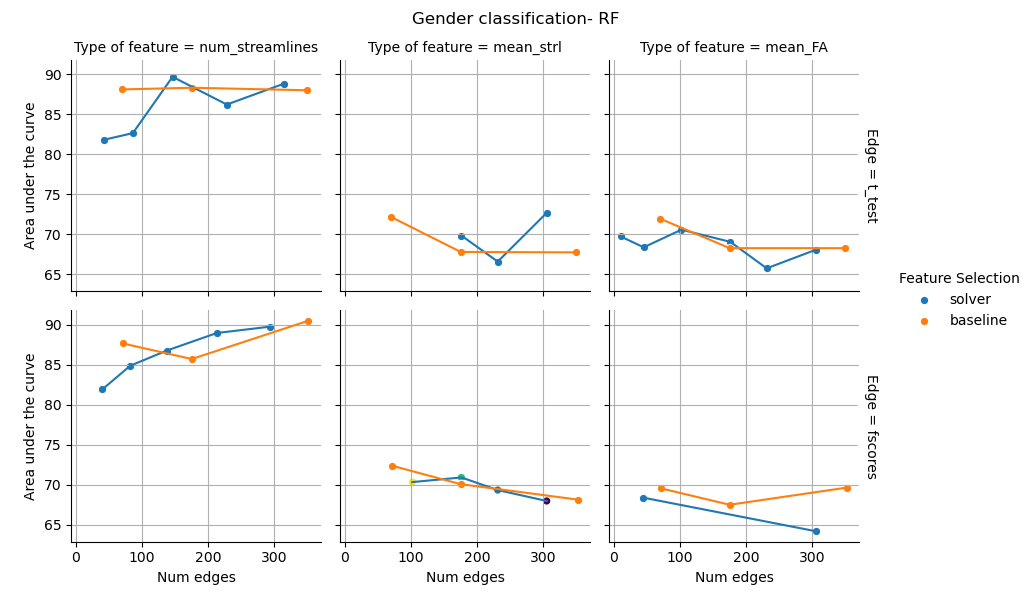
\includegraphics[width = \textwidth]{images/comparison_roc_auc_RF.png}
    \caption{Caption}
    \label{fig:rfgender}
\end{figure}
\fi





Judging on the basis of the area under the curve for gender based classification, it is best to compare feature wise.

Consider the mean FA feature first, for this feature the solver based approach does better than or equivalently well as the baseline when the number of edges preserved is small. This is not surprising since the number of edges preserved is a function of the number of nodes specified by the solver based technique. When a specified number of edges would be wanted to be preserved then the features corresponding to only those nodes will be preserved, this makes an inherent bias into which features will be preserved by the solver. Since all one node might have multiple highly relevant performance features but we want to preserve a given number of nodes, so the other less performing feature might be selected since a particular node has to be selected.



\section{Classification}

\begin{figure}
    \centering
    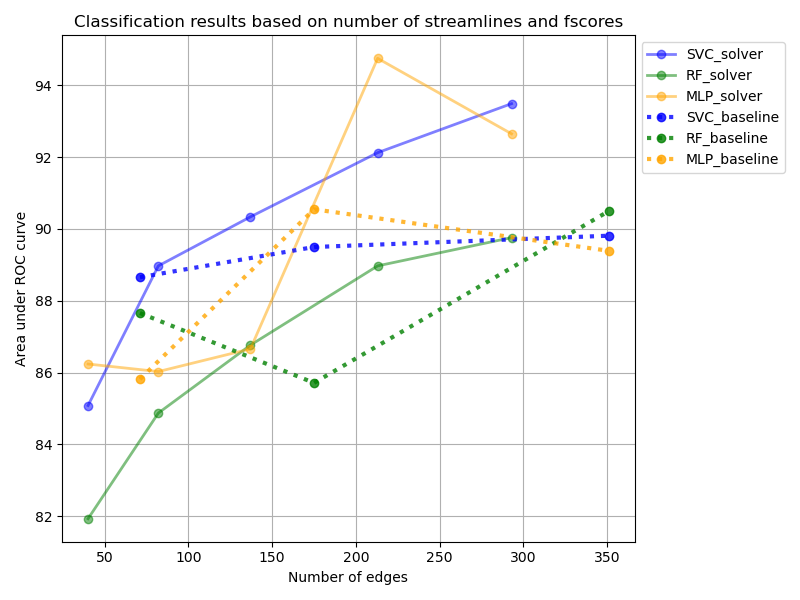
\includegraphics[width=0.8\textwidth]{images/select_clf_auc_gender.png}
    \caption{Comparison of area under the ROC curve for gender classification on the independent test set. The performance of three classifiers Support Vector Machines, Random Forest and Multilayer perceptron on the basis of features filtered according to the solver and baseline experiments respectively.}
    \label{fig:clf_solver results}
\end{figure}

\begin{figure}
    \centering
    %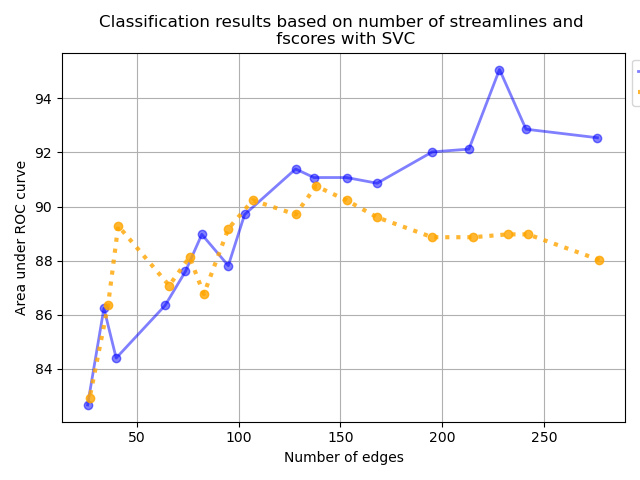
\includegraphics[width=0.8\textwidth]{images/select_clf_auc_gender_2_svc.png}
    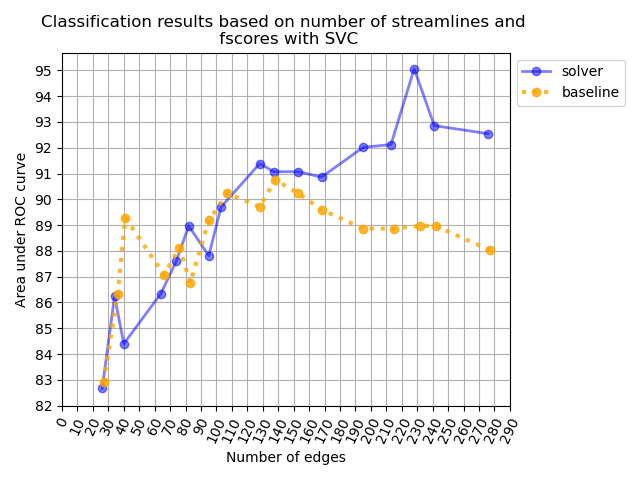
\includegraphics[width=0.8\textwidth]{images/select_clf_auf_gender_2_scaled.png}
    \caption{Classification using solver and baseline for the exact same number of features selected in each case.}
    \label{fig:svcgender}
\end{figure}

On closely analyzing the behaviour from the curve as viewed above. The SVM based classification produced more stable results. More data points were then sampled. This time the number of edges preserved by the solver was used to decide the parameter top $k$ percentile of features to be preserved in the baseline analysis. From the \autoref{fig:svcgender}, it became clear that after a cutoff number of edges, i.e. precisely 137 (obtained from the function in \autoref{fig:fun_num_edges} and the preprocessed files, the solver definitely does better than the baseline analysis. Even for the number of edges below 137, the results remain comparable but more interpretable. So for the solver, the number of nodes for gender classification that definitely yields better results than the baseline experiments after 137 edges. Corresponds to 20 nodes i.e. ($137 \approx 0.285* 400 + 1.467(20) - 3.888 = 114 + 29.34-3.88 = 139.46$). So for below 20 nodes there is a bit of a compromise for classifier performance but increased interpretability and ease of visualization. While for higher than 20 nodes, there is a decrease in interpretability but an increase in classifier performance.

\subsection{Best parameters}
For our configuration using Multilayer perceptron for the solver based reduction, classification of gender using the feature selection technique of fscores and refit metric balanced accuracy. Baseline based on 5\% of features. The parameters for the best estimator of the cross validation turn out to be the same, this justifies that the solver based method works better than the baseline method when it comes to classification accuracy and also leads to an increase in the interpretability.
% Best estimator {'solver': 'adam', 'learning_rate': 'adaptive', 'hidden_layer_sizes': (50, 100, 100, 50), 'alpha': 0.05, 'activation': 'relu'}
% ('MLP', 'Gender', 'random', 'fscores', 'baseline', 'num_streamlines', 5, 'balanced_accuracy', False)
%Bet estimator {'solver': 'adam', 'learning_rate': 'adaptive', 'hidden_layer_sizes': (50, 100, 100, 50), 'alpha': 0.05, 'activation': 'tanh'}
\begin{table}[b]
    \centering
    \begin{tabular}{|c|c|c|}
        \specialrule{0.1em}{0.05em}{0.05em}
        Hyperparameter & Solver & baseline \\
        \hline
        solver & adam & adam\\
        \hline
        hidden layer size &  50,100,100, 50 & 50,100,100,50\\
        \hline
        activation function & relu & tanh\\
        \hline
        alpha & 0.05 & 0.05\\
        \hline
        learning rate & adaptive & adaptive\\
        \hline
    \end{tabular}
    \caption{Cross validation parameters for MLP trained for gender classification. The parameters which give the best area under the curve for the use case mentioned in the section above have been presented}
    \label{tab:MLP best params}
\end{table}
The SVM seemed to give most stable results and the maximum area under the curve given by the for gender classification is 95\% for number of nodes 26. These parameters are for the solver based experiments and classifier SVC. For the best estimator with the baseline experiments the around 138 edges does the best with 91\% AUC so the parameters for that are presented in the table. 
%Best estimator {'C': 5.918565074193836, 'class_weight': 'balanced', 'gamma': 0.0004643818614121193, 'kernel': 'rbf'}
%Best estimator basline {'C': 0.5229762127721259, 'class_weight': None, 'gamma': 0.008523831363402392, 'kernel': 'rbf'}

\begin{table}[b]
    \centering
    \begin{tabular}{|c|c|c|}
        \specialrule{0.1em}{0.05em}{0.05em}
        Hyperparameter & Solver & baseline \\
        \hline
        C & 5.9 & 0.522\\
        \hline
        Gamma &  4e-4 &  8e-4\\
        \hline
        kernel &  rbf & rbf\\
        \hline
        class weight & balanced & None\\
        \hline
    \end{tabular}
    \caption{Cross validation parameters for SVC trained for gender classification. The parameters which give the best area under the curve for the use case mentioned in the section above have been presented}
    \label{tab:CSV best parameters}
\end{table}

\end{document}
